\section{Historical Results: Context Only}
\subsection{Full-horizon tracking and retained failure}
The J archive contains ten validation and ten final V4 trials, each reported as completing the original thirty-second task. These belong to the earlier guarded contact domain and are historical context, not extra replications of the later adapter. Under the L contact correction, three development and three confirmation V4 trials completed thirty seconds with sixteen of sixteen tracking windows. Confirmation vector RMSE values were $0.04850230$, $0.04247506$, and $0.04842782$ m; their mean was $0.04646839$ m. The corresponding mean modal energy was approximately $75.92735$ microjoules across those three trials.\claim{C15}

This evidence has a counterexample. The known M stress context physically continued for thirty seconds but passed only fifteen windows. Its vector RMSE was $0.05251372$ m, yet the first window's minimum synchronous error was $0.10230571$ m, above the $0.10$ m tolerance.\claim{C16} A favorable overall RMSE did not override the failed window. The archive thus supports recorded V4 completion, not universal success across represented terrain resets. No missing teacher or PPO thirty-second trial is filled using the V4 result.

The K comparison includes V2, V3, feedforward, V4, BC, Standard PPO, and KL-regularized policy interfaces, but it also contains contact-censored rough trials and policies transferred from different training tasks. The evidence registry preserves attempted duration, completion, information regime, and termination. These records are useful for diagnosing reference-interface mismatch, but do not form a clean final all-controller ranking. PID balance-only behavior is likewise excluded from a trajectory-tracking superiority statement.
\begin{table*}[t]
\centering\small
\caption{L V4 30-s trials, n=3 DEV and n=3 confirmation. Each row is one independent reset/terrain context; original frozen metric and contact L. Sources: L evaluation\_results.json.}
\label{tab:full_horizon}
\begin{tabular}{llllll}
\hline
Seed & Split & XY RMSE (m) & Mean E (uJ) & Torque RMS (Nm) & Nodes \\
\hline
1800101 & DEV & 0.045243 & 111.625 & 1.8876 & 16/16 \\
1800102 & DEV & 0.048255 & 118.826 & 1.8424 & 16/16 \\
1800103 & DEV & 0.047759 & 63.010 & 1.9050 & 16/16 \\
1801001 & confirmation & 0.048502 & 64.792 & 1.9216 & 16/16 \\
1801002 & confirmation & 0.042475 & 36.632 & 1.9119 & 16/16 \\
1801003 & confirmation & 0.048428 & 126.358 & 1.8455 & 16/16 \\
\hline
\end{tabular}
\end{table*}

\begin{figure*}[t]\centering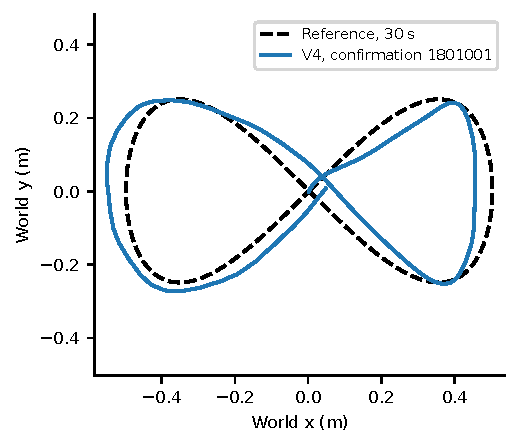
\includegraphics[width=.39\textwidth]{figures/fig02.pdf}\hfill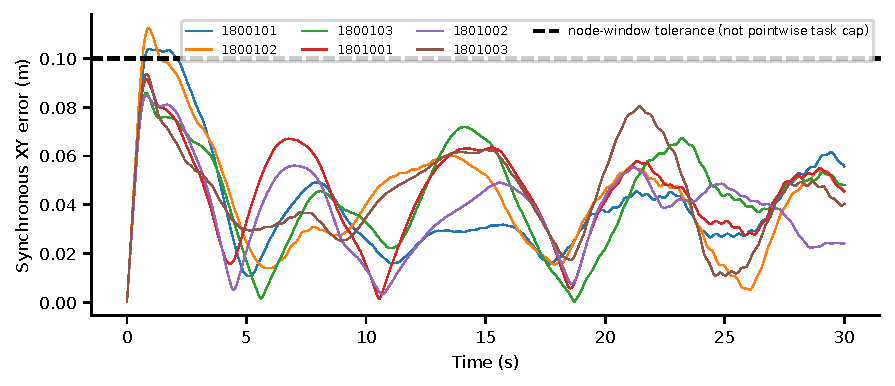
\includegraphics[width=.56\textwidth]{figures/fig03.pdf}\caption{L full-horizon V4 trajectory and six tracking-error histories. Confirmation seed1801001 is the illustrated path. Development and confirmation are not pooled for checkpoint selection.}\end{figure*}
\begin{figure*}[t]\centering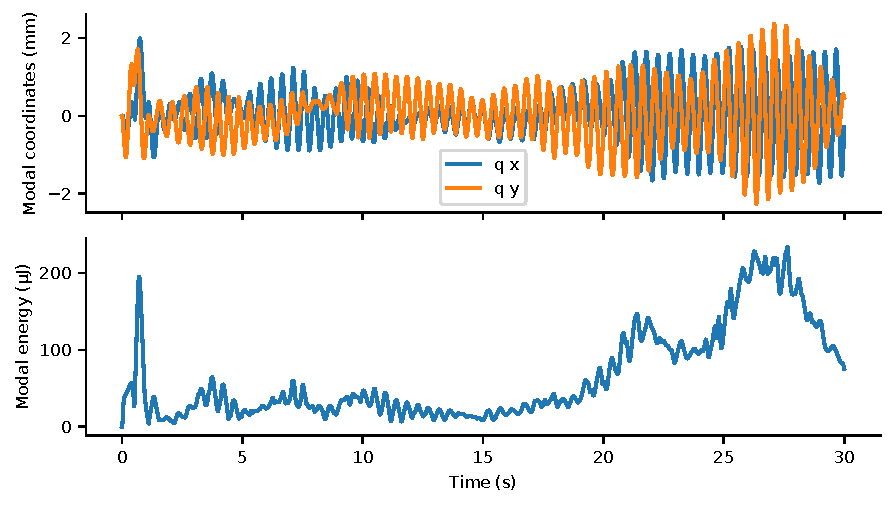
\includegraphics[width=.48\textwidth]{figures/fig04.pdf}\hfill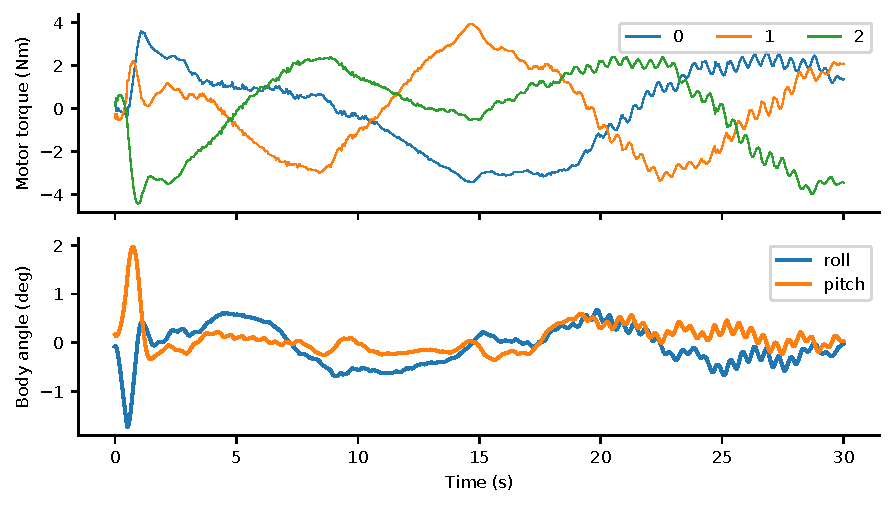
\includegraphics[width=.48\textwidth]{figures/fig05.pdf}\caption{Modal, actuator, and balance histories from the same archived full trial. The liquid curves represent generalized coordinates, not a reconstructed water surface.}\end{figure*}
\begin{figure}[t]\centering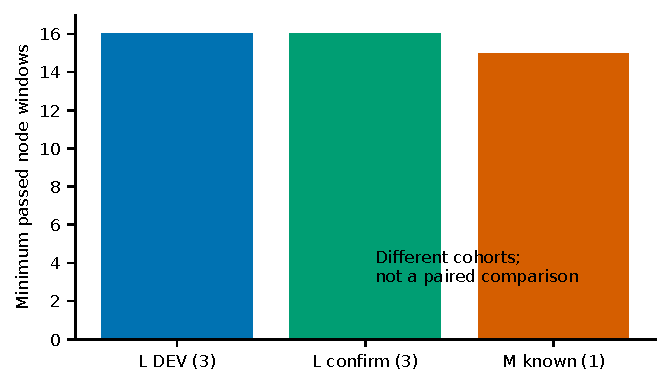
\includegraphics[width=\columnwidth]{figures/fig06.pdf}\caption{Full-duration evidence includes an M known stress failure. Bars show minimum passed windows within each labeled cohort, not statistical success probabilities.}\end{figure}

\subsection{Teacher feasibility and horizon dependence}
The U teacher recovered a known context that earlier stopped because a relative tracking-performance budget was exhausted. The earlier candidates remained physically admissible; the stop did not establish uncontrollability of the plant. U explicitly allows labeled performance-degraded continuation while preserving absolute task and physical guards. Its three fresh one-second confirmation contexts reduced mean modal energy relative to paired V4 by approximately $3.287\%$, $3.226\%$, and $7.436\%$.\claim{C17} For three successes in three registered contexts, the archived exact binomial 95\% interval is [0.2924,1]. The per-seed mean energy reduction has an assumption-dependent 95\% t interval spanning approximately [-1.345,10.645] percentage points. These short paired cases do not establish a robust full-task teacher advantage.

The same U FRESH\_1 context provides a particularly important negative result. Mean energy increased by $5.6136\%$ over the first three seconds but decreased by $17.6206\%$ over five seconds. The saved trajectories share an identical first-three-second native prefix. The energy ratio over the added three-to-five-second interval was approximately $0.496627$.\claim{C18} Thus the change in aggregate sign reflects window-dependent modal exchange, not two independent replications or a retuned fluid damping coefficient. The four-mode supervisor supports tested continuation, but no accepted thirty-second teacher demonstration or formal recursive-feasibility proof follows.

Measured U decision costs averaged approximately $2.801$ s, with a $3.380$ s 95th percentile, for a nominal $0.2$ s decision hold.\claim{C19} These costs include the recorded offline search path and cannot be presented as real-time deployment performance. Wider horizons were not inferred from unmeasured extrapolation, and the optional thirty-second U experiment remained unopened.
\begin{figure}[t]\centering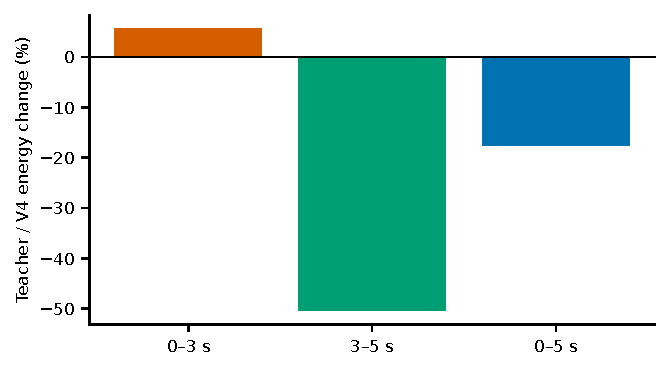
\includegraphics[width=\columnwidth]{figures/fig07.pdf}\caption{U energy effects depend on the observed time window. These windows are correlated portions of one context.}\end{figure}

\subsection{Learning pipeline and structured exploration}
The V pilot and W continuation supplied evidence of policy updates and extensive rollout diagnostics, but did not establish a consistent improvement over V4. X subsequently found useful short held-action perturbations in selected states. Its $0.30$ s action-hold experiment demonstrates local control opportunity; it does not show that independent policy samples every $10$ ms reproduce that opportunity.

Y increased analytic initial probability in small boxes around previously useful action centers by approximately $654$--$1,352$ times relative to the initial Standard Gaussian. The boxes use a $0.025$ normalized-delta half-width.\claim{C20} Their centers have local causal evidence, but the entire volume and every resulting action sequence were not validated as beneficial. The mixture simultaneously changes variance and geometry, preventing attribution to multimodality alone.

All four Y runs completed the registered transition count. The archive contains twenty checkpoint files and 128 rollout buffers. The independent verifier reconstructed GAE with maximum gap approximately $8.94\times10^{-8}$ and replayed representative old log probabilities with maximum gap approximately $1.55\times10^{-6}$. No NaN, ROM, contact, or torque failure was recorded in the completed training runs.\claim{C21} These are implementation and domain-admissibility observations, not success rates for unseen terrain.

The matched final contrasts are unfavorable to a general Mixture energy claim. Mixture mean energy exceeded Standard in all four crossed development cells, by approximately $0.0714$--$0.1726\%$. Seed2271001 also had slightly worse tracking under Mixture. Seed2271002 improved tracking by approximately $22.883$ and $26.808$ micrometres relative to Standard while retaining the energy disadvantage.\claim{C22} Descriptive trade-offs are therefore appropriate; statistical superiority is not.
\begin{table*}[t]
\centering\small
\caption{Y final Mixture relative to matched Standard. n=2 training seeds crossed with two development cases; four cells are not four independent training replications. Source: tables/paired\_final.csv.}
\label{tab:mixture}
\begin{tabular}{llll}
\hline
Training seed & DEV & Energy change (\%) & RMSE change (um) \\
\hline
2271001 & DEV\_1 & 0.089412 & 6.934065 \\
2271001 & DEV\_2 & 0.071389 & 2.244753 \\
2271002 & DEV\_1 & 0.156332 & -22.882605 \\
2271002 & DEV\_2 & 0.172634 & -26.807697 \\
\hline
\end{tabular}
\end{table*}

\begin{figure*}[t]\centering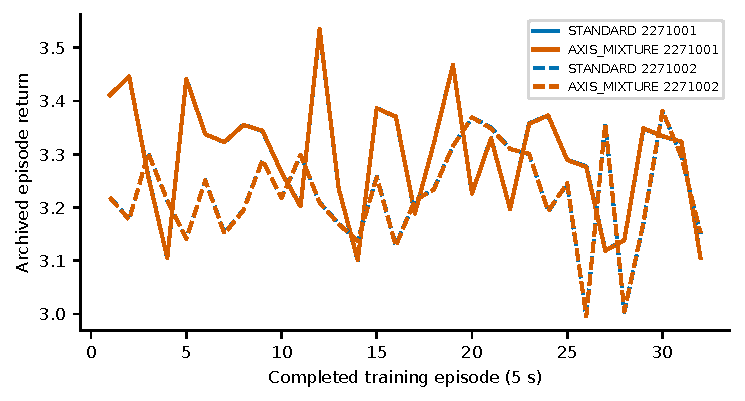
\includegraphics[width=.45\textwidth]{figures/fig08.pdf}\hfill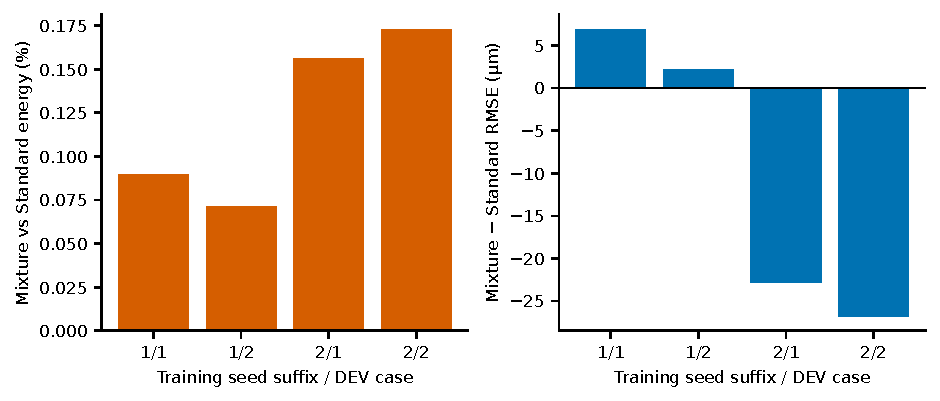
\includegraphics[width=.51\textwidth]{figures/fig09.pdf}\caption{Y archived return curves and matched final contrasts. Curves are unsmoothed completed-episode returns; neither curve points nor DEV cells are independent training replications.}\end{figure*}

\subsection{Selected development effect and numerical checks}
The registered selection rule chose Mixture seed2271002 relative to V4. Its two one-second DEV tracking gains were approximately $25.618$ and $28.788$ micrometres, with energy changes $-0.08916\%$ and $-0.14175\%$.\claim{C23} These are small selected effects, not an all-seed result. The second Mixture seed did not reproduce an energy benefit over V4.

For the selected DEV1 condition, native refinement from $2$ to $1$ and $0.5$ ms retained the effect signs. The paired RMSE effect varied by approximately $0.02339$ micrometres and the energy effect by $1.11374\times10^{-9}$ J over these sampled resolutions.\claim{C24} This supports local numerical distinguishability, not a rigorous error bound. It also does not replace paired refinement of every Standard-versus-Mixture contrast or of a full thirty-second trajectory.

Conditional three-second comparisons completed both DEV task and physical guards. Energy changed by $-0.13651\%$ and $+0.18644\%$ relative to V4, while tracking improved by approximately $43.371$ and $42.829$ micrometres. The mean energy change was $+0.02497\%$, so the aggregate benefit gate failed and five-second evaluation was not opened.\claim{C25} This is a benefit failure, not a physics failure or incomplete three-second trajectory. No PPO thirty-second completion is claimed.
\begin{table*}[t]
\centering\small
\caption{Selected Mixture Y vs V4, conditional 3-s DEV evaluation. Selection used the same DEV pool; not fresh confirmation. Both pairs completed task and physical guards; aggregate benefit gate failed.}
\label{tab:longer}
\begin{tabular}{llll}
\hline
Case & Horizon (s) & Energy change (\%) & RMSE change (um) \\
\hline
DEV\_1 & 3 & -0.136507 & -43.370555 \\
DEV\_2 & 3 & 0.186440 & -42.829230 \\
\hline
\end{tabular}
\end{table*}

\begin{table*}[t]
\centering\small
\caption{Y selected DEV1 paired active-loop timestep sensitivity. n=1 selected policy/context at three timesteps; not independent samples.}
\label{tab:numerical}
\begin{tabular}{lll}
\hline
Timestep (ms) & Energy change (\%) & RMSE change (um) \\
\hline
2.0 & -0.089156 & -25.617900 \\
1.0 & -0.089773 & -25.634636 \\
0.5 & -0.090489 & -25.641288 \\
\hline
\end{tabular}
\end{table*}

\begin{figure}[t]\centering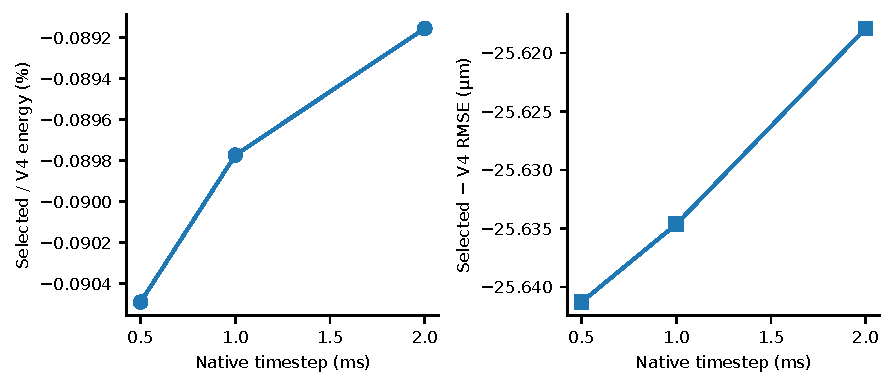
\includegraphics[width=\columnwidth]{figures/fig10.pdf}\caption{Selected Y DEV1 active-loop sensitivity at three native steps. Sensitivity points share the same selected policy and context.}\end{figure}
